\chapter{Проведение экспериментов}\label{ch:ch4}
В этой главе будут рассмотрены проведённые эксперименты по поиску достаточного набора значений для описания состояния робота $s \in S$, а также по подбору значений функции награды $r$, которые возвращает среда в ответ на действия агента. 

Для обучения агента всё время использовался алгоритм tqc \cite{kuznetsov2020controlling} со стандартными настройками. Прочие методы обучения не рассматривались, так как они влияют лишь на скорость сходимости к оптимальной модели. Но вид оптимальной модели определяется при помощи свойств внешней среды в симуляторе, а также функции награды $r$. Поэтому фокус в данной работе именно на подборе этих параметров.

\section{Начальный запуск с ограничением угла поворота головы}\label{sec:ch1/sec5}
Этот эксперимент был первым запуском, который положил направление дальнейшего развития. При выборе множества состояний я руководствовался экономией ресурсов, поэтому включил минимально возможный набор: углы сервомоторов и положение IMU. Робот награждался за скорость вдоль целевого направления, а также сессия прекращалась, если какой-то из углов поворота головы имел высокое абсолютное значение~--- таким образом получалось предсказывать падение робота и не тратить время на лишние итерации симуляции.
\subsection{Конфигурация}\label{sec:ch1.1/sec5}

Множество состояний $S = S_{joint\_state} \times S_{imu\_quat}$. Где $S_{joint\_state} = [-1, 1]^{13}$~--- множество возможных нормированных значений углов моторов ног и бедра, 6 на каждую ногу и один сервомотор бедра. А $S_{imu\_quat} = [0, 1]^4$~--- значения кватернионов поворота IMU.

Множество Действий $A = [-1, 1]^{14}$ соответсвует набору активных при ходьбе сервомоторов. Каждое действие задаёт целевой угол поворота, к которому сервомотор стремится с максимально допустимой для него скоростью. Множество действий можно было определять также и через задание скоростей сервомоторов, но в текущей работе был выбран подход с целевыми положениями, так как такой же подход использовался и в базовой модели. 

В качестве функции награды использовалась линейная скорость в метрах в секунду вдоль оси целевого направления $V_x$, а также дополнительная награда 0.001 за то, что робот не упал. Скорость $V_x$ считалась при помощи замера изменения положения IMU за 20 итераций выполнения симуляции, поделенного на $\frac{20}{30}$, так как за секунду симуляция считала 30 итераций. Проверка на падение выполнялась при помощи сравнения абсолютных углов отклонения IMU относительно глобальных координат с 45\%~--- при превышении этого порога робот считался упавшим и симуляция прекращалась. Таким образом выбранная награда стимулировала робота не падать, так как в таком случае робот получил бы ограниченную награду, а также двигаться вперёд, чтобы получить дополнительную награду за передвижение. 


\subsection{Результаты}\label{sec:ch1.2/sec5}
В итоге запуска процедуры обучения дисконтированная сумма наград не росла, что было явным признаком проблем с обучением. Воспроизведение полученной модели поведения показало, что робот дёргался на месте, задавая значения поворотов сервомоторам около нуля. Это мне показалось следствием того, что выбранное множество состояний не обеспечивает марковское свойство для модели, а поэтому при обучении модель не может идентифицировать своё текущее положение, и соответственно не может выбрать нужное целевое действие.

\section{Устойчивое передвижение робота}\label{sec:ch2/sec5}
После первого запуска было решено использовать всю доступную информацию для определения состояния робота. Единственное ограничение, которое должно выполняться~--- любая информация, которую будет использовать модель для предсказания действия, должна быть доступна на реальном роботе. Например, нельзя в состоянии передавать абсолютные координаты всех частей робота, так как такую информацию на механическом роботе никак не получить: для этого нужно знать, в какой координате робот касается поверхности земли, что невозможно рассчитать в реальном мире с достаточной точностью. Поэтому к уже имеющимся в состоянии углам моторов и кватернионам я добавил угловые скорости вращения сервомоторов, моменты силы моторов и угловые скорости поворота IMU в углах эйлера.

\subsection{Конфигурация}\label{sec:ch2.1/sec5}

Множество состояний $S = S_{joint\_state} \times S_{join\_velocity} \times S_{joint\_torque} \times S_{imu\_quat} \times S_{imu\_velocity}$. Где $S_{joint\_state} = [-1, 1]^{13}$ и $S_{imu\_quat} = [0, 1]^4$~--- определены в предыдущем эксперименте. $S_{join\_velocity} = [-1, 1]^{13}$~--- скорость изменения значений поворотов сервомоторов, указывается относительно максимальных значений скоростей, где $-1$ соответствует максимальной скорости по часовой стрелки, а $1$ соответсвует максимальной скорости против часовой стрелки. $S_{joint\_torque} = \mathbb{R}^{13}$~--- моменты силы в текущую итерацию выполнения симуляции. Эти значения было решено не нормировать, так как максимальные значения неизвестны заранее. $S_{imu\_velocity}=\mathbb{R}^3$~--- скорости поворотов углов эйлера IMU в градусах в секунду. Это состояние должно помогать определять направление движение туловища во время ходьбы.

Множество возможных действий $A$ и функция награды $r$ остались прежними.


\subsection{Результаты}\label{sec:ch2.2/sec5}

В итоге при такой конфигурации модель выучила алгоритм, который обеспечивал стабильное передвижение вперёд см. рисунок ~\cref{fig:robot_4.2}. Этот результат оказался неудовлетворительным, так как робот садится достаточно низко. В такой позе происходит пересечение составляющих деталей робота~--- такое состояние нельзя считать допустимым на реальном роботе. Также движение обеспечивается за счёт высокочастотной вибрации стоп, что также невозможно на физической модели, так как в таком случае сервомоторы быстро бы перегрелись и вышли из строя. Получается, что полученная конфигурация хоть и обеспечивает сходимость процедуры обучения, но всё равно сходится к нереалистичной модели ходьбы. В таком случае нужно конфигурировать функцию награды и настраивать свойства окружения в симуляции.


\begin{figure}[ht]
    \centerfloat{
        \hfill
        \subcaptionbox[List-of-Figures entry]{\label{fig:robot_4.2.1}}{%
            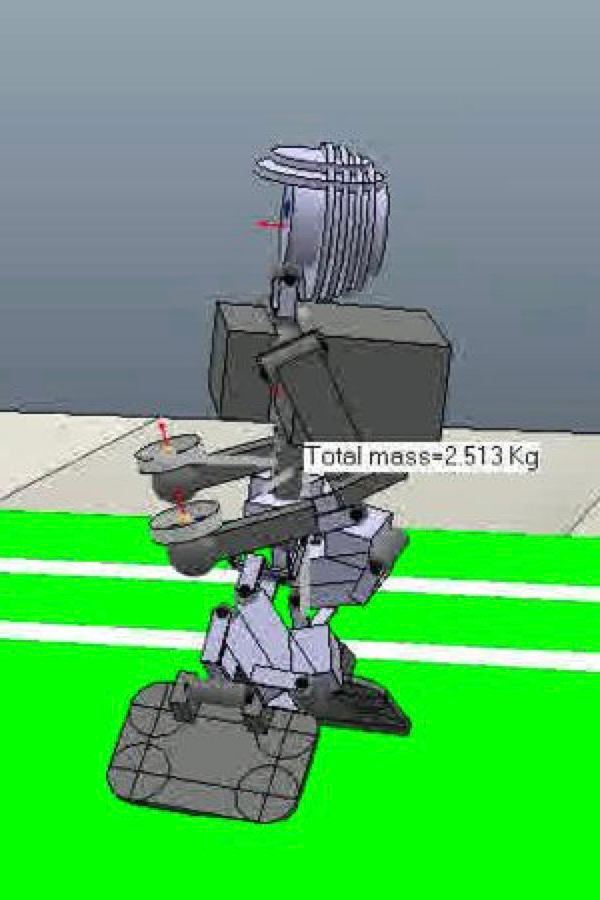
\includegraphics[width=0.3\linewidth]{images/robot_4.2.1.jpg}}
        \hfill
        \subcaptionbox{ \label{fig:robot_4.2.2}}{%
            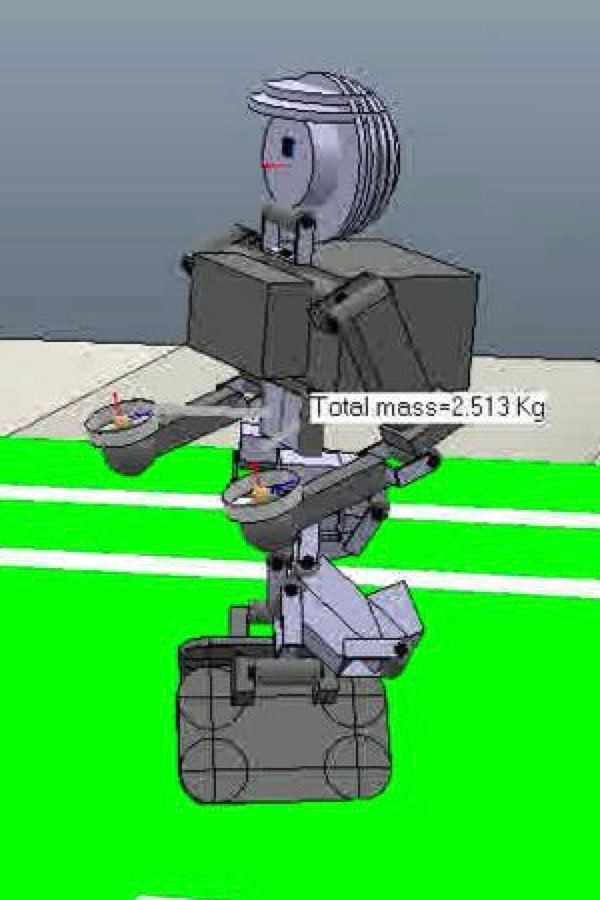
\includegraphics[width=0.3\linewidth]{images/robot_4.2.2.jpg}}
        \hfill
        \subcaptionbox[List-of-Figures entry]{\label{fig:robot_4.2.3}}{%
            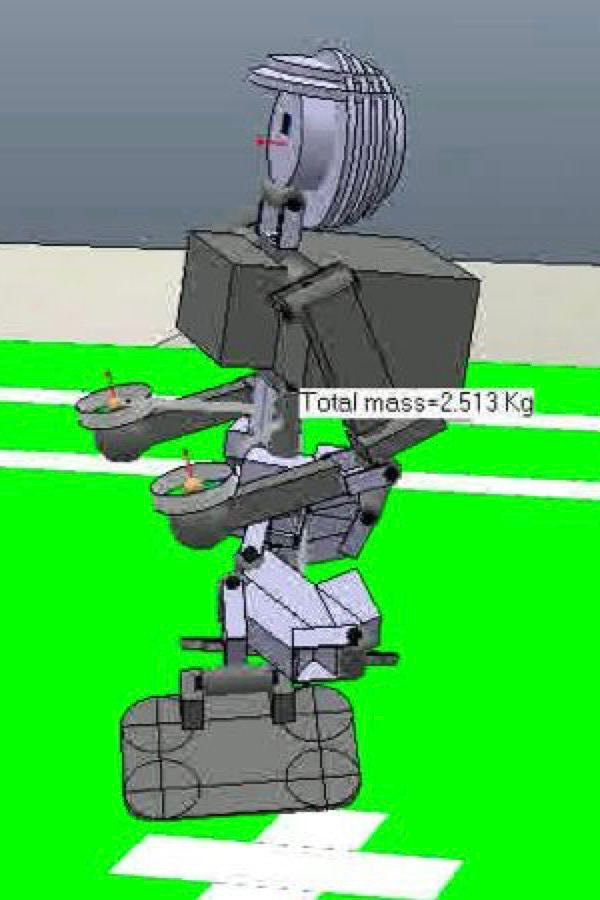
\includegraphics[width=0.3\linewidth]{images/robot_4.2.3.jpg}}
        \hfill
    }
    \caption[Пример первого устойчивого передвижения]{Пример первого устойчивого передвижения}\label{fig:robot_4.2}
\end{figure}


\section{Движение без самопересечения}\label{sec:ch3/sec5}
В этом эксперименте были устранены недочёты в настройке среды, которые позволяли роботу достигать состояний с самопересечением. Во-первых для каждого сервомотора были просчитаны максимальный и минимальный углы поворотов, которые не мешали бы базовой ходьбе. А также была добавлена проверка на самопересечения при помощи встроенных методов симуляции. Теперь симуляция входит в терминальное состояние не только, когда робот начинает падать, но также когда у робота какие-либо части модели пересекаются. Такие ограничения должны обеспечить обучение более реалистичных движений.

\subsection{Конфигурация}\label{sec:ch3.1/sec5}

Множество состояний осталось прежним благодаря тому, что изначально мы использовали значения относительно максимально/минимально возможных. Это позволяет менять свойства симуляции без переопределения входных параметров у модели.

Множество возможных действий $A$ осталось прежним.

Функция награды $r$ осталась прежней, только теперь эпизод симуляции прерывается дополнительно, когда симуляция определяет самопересечение составляющих робота.

\subsection{Результаты}\label{sec:ch3.2/sec5}

В результате была получена модель см. рисунок~\cref{fig:robot_4.3}, которая передвигается в положении с выпрямленными ногами, двигается быстрее базовой модели в заданном направлении. Но полученная модель движения всё равно не выглядит реалистично, так как робот передвигается на одной ноге, а значит сервомотор стопы должен испытывать большое давление, что привело бы к перегреву на реальном роботе. Также стопа во время движения изогнута и касается земли лишь ребром. Движение обеспечивается поочерёдным поднятием начала и конца стопы, а также наклоном робота вперёд. Данная походка также является неустойчивой, так как в симуляции еще не учтены неровности поверхности, которые могли бы нарушить баланс модели и привести к падению робота.

\begin{figure}[ht]
    \centerfloat{
        \hfill
        \subcaptionbox[List-of-Figures entry]{\label{fig:robot_4.3.1}}{%
            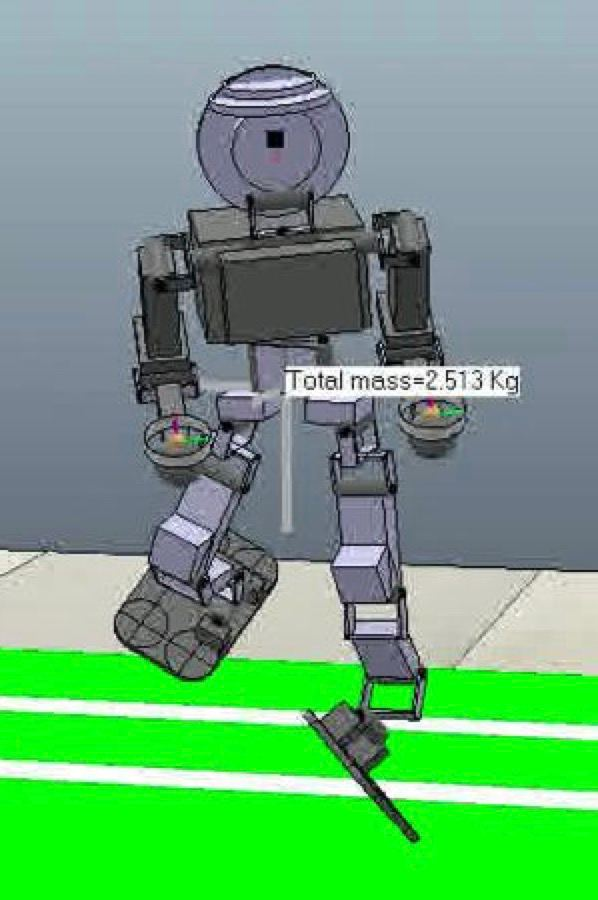
\includegraphics[width=0.3\linewidth]{images/robot_4.3.1.jpg}}
        \hfill
        \subcaptionbox{ \label{fig:robot_4.3.2}}{%
            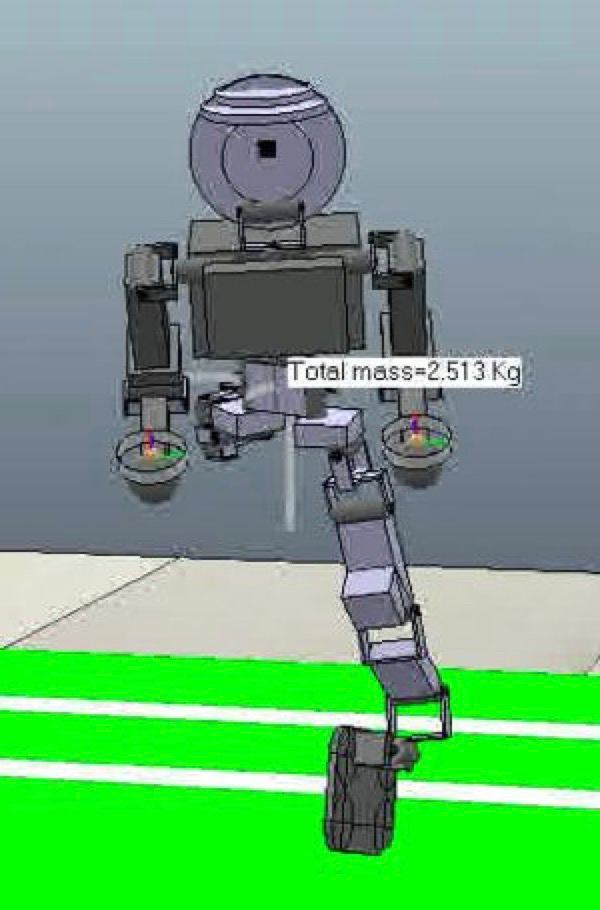
\includegraphics[width=0.3\linewidth]{images/robot_4.3.2.jpg}}
        \hfill
        \subcaptionbox[List-of-Figures entry]{\label{fig:robot_4.3.3}}{%
            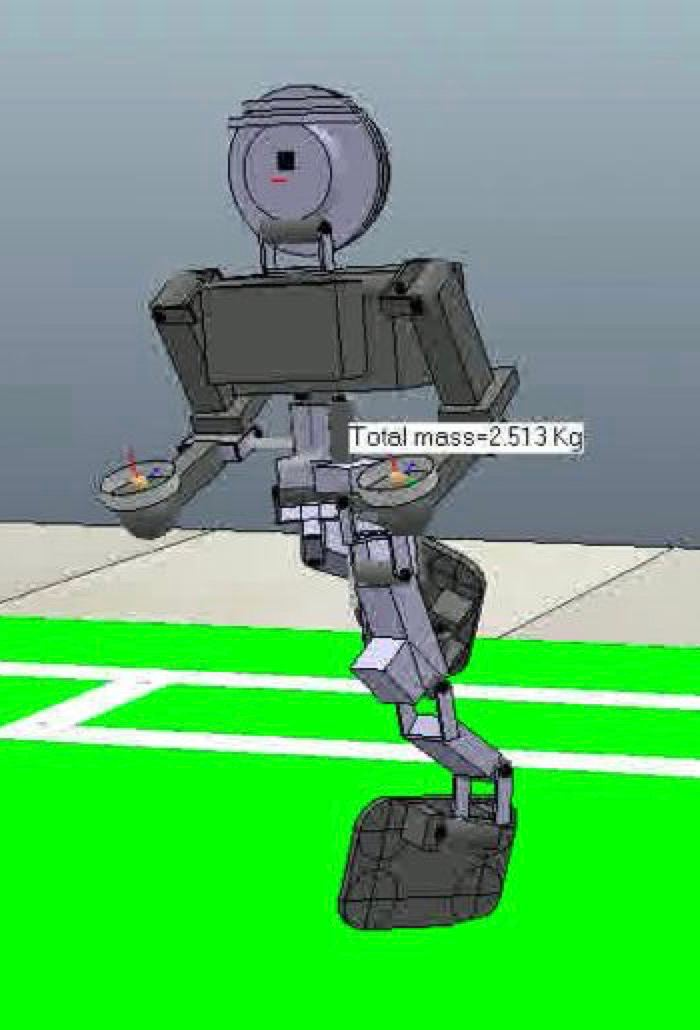
\includegraphics[width=0.31\linewidth]{images/robot_4.3.3.jpg}}
        \hfill
    }
    \caption[Пример движения без самопересечения]{Пример движения без самопересечения}\label{fig:robot_4.3}
\end{figure}


\section{Ходьба с ограниченной нагрузкой на сервомоторы}\label{sec:ch4/sec5}
В этом эксперименте была предпринята попытка избавиться от избыточного напряжения в определенных сервомоторах. Для того, чтобы формализовать это требование, нужно понять, из-за чего возникают такого рода нагрузки. Опыт показал, что они возникают, когда сервомотор стремится совершить оборот со встречной нагрузкой, создающей ответное сопротивление. В реальном роботе это происходит, например, когда робот стоит на одной ноге или пытается совершить движение конечностью, которая упирается в препятствие. Физической характеристикой силы крутящего момента является момент силы. Это значение является доступным для считывания на реальном роботе, поэтому было решено использовать момент силы в качестве характеристики перегрева сервомоторов.

\subsection{Конфигурация}\label{sec:ch4.1/sec5}
Множество состояний в этом эксперименте остаётся прежним, так как ранее хорошо показало себя в обучении модели.  $S = S_{joint\_state} \times S_{join\_velocity} \times S_{joint\_torque} \times S_{imu\_quat} \times S_{imu\_velocity}$.

Множество возможных действий $A$ осталось прежним

Функция награды немного изменилась: $r = V_x + 0.001 - 4 \frac{||J||_1}{J_\max}$. Добавилась отрицательная награда $\frac{||J||_1}{J_\max}$~--- штраф за высокие относительные нагрузки, где $J$ является вектором моментов сил для моторчиков, а $J_\max$ является максимальным допустимым моментом для выбранной модели сервомоторов. Параметр $J_\max$ подбирается исходя из физических свойств и рекомендаций по эксплуатации сервомоторов. 


\subsection{Результаты}\label{sec:ch4.2/sec5}
В результате робот научился стоять неподвижно на месте, так как штраф за нагрузки оказался сильнее, чем награда за скорость см. рисунко~\cref{fig:robot_4.4} . Такой результат наводит на мысль, что нужно использовать не абсолютные параметры, такие как коэффициент $-4$ перед штрафом, а относительные коэффициенты, сумма которых будет равняться единице. Такой подход позволит проще переносить выбранную награду на другие модели роботов.
\begin{figure}[ht]
    \centerfloat{
        \hfill
        \subcaptionbox[List-of-Figures entry]{\label{fig:robot_4.4.1}}{%
            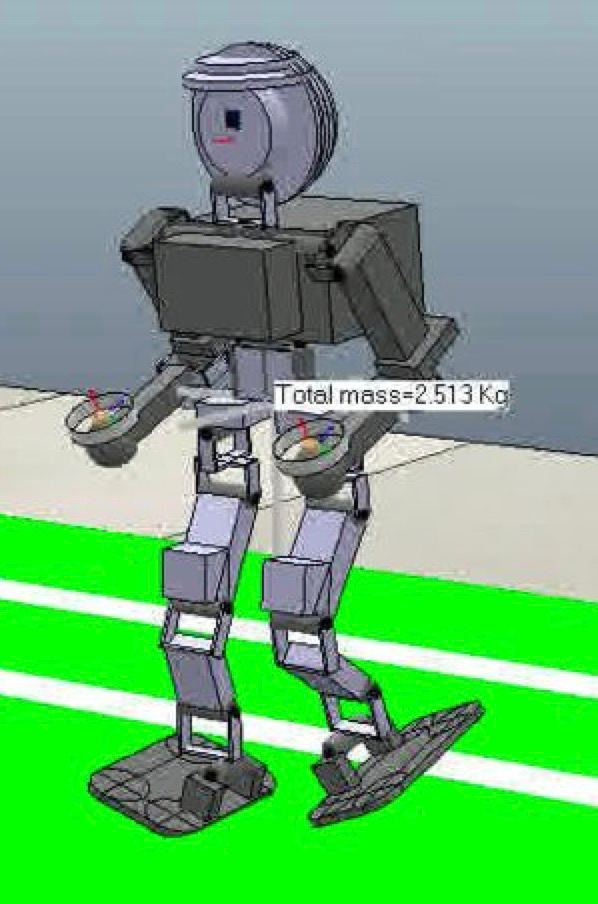
\includegraphics[width=0.3\linewidth]{images/robot_4.4.1.jpg}}
        \hfill
        \subcaptionbox{ \label{fig:robot_4.4.2}}{%
            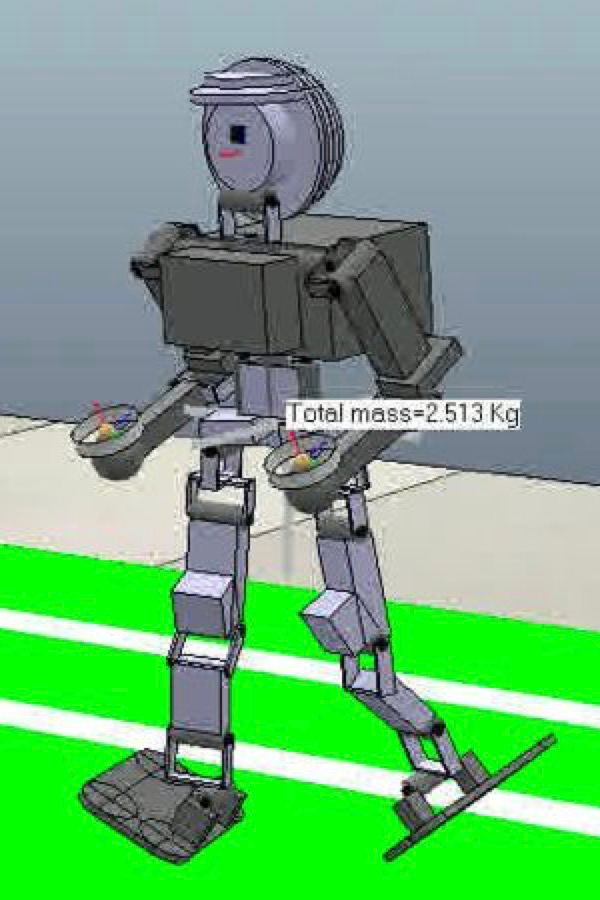
\includegraphics[width=0.3\linewidth]{images/robot_4.4.2.jpg}}
        \hfill
        \subcaptionbox[List-of-Figures entry]{\label{fig:robot_4.4.3}}{%
            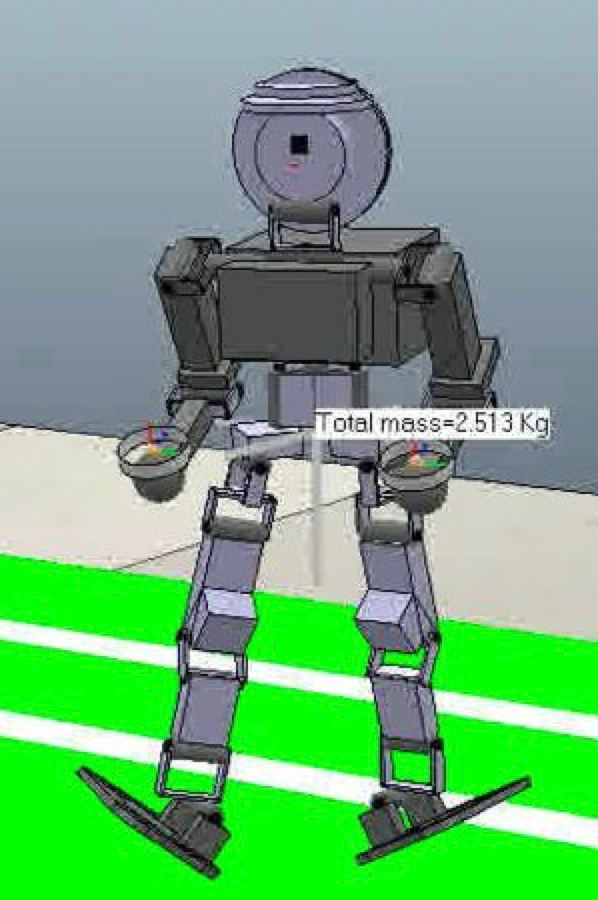
\includegraphics[width=0.31\linewidth]{images/robot_4.4.3.jpg}}
        \hfill
    }
    \caption[Пример ходьбы с ограниченной нагрузкой на сервомоторы]{Пример ходьбы с ограниченной нагрузкой на сервомоторы}\label{fig:robot_4.4}
\end{figure}


\section{Пробежка с унифицированной функцией награды}\label{sec:ch5/sec5}
В этом эксперименте было решено унифицировать функцию награды, чтобы она принимала значения от 0 до 1. Но особенность в том, что для этого понадобилось унифицировать все составляющие этой суммы, а полученный ряд сложить с весами, сумма которых равна единице. Этот метод помог определить глобальные параметры, которые определяются при помощи характеристик физической модели робота, а значит могут быть легко адаптированы под новые модели.

\subsection{Конфигурация}\label{sec:ch5.1/sec5}
Множество состояний в этом эксперименте остаётся прежним, так как ранее хорошо показало себя в обучении модели.  $S = S_{joint\_state} \times S_{join\_velocity} \times S_{joint\_torque} \times S_{imu\_quat} \times S_{imu\_velocity}$.

Множество возможных действий $A$ осталось прежним

Функция награды $r$ теперь равняется сумме $0.4R_{velocity} + 0.4R_{force} + 0.2R_{stable}$, где $R_{velocity}, R_{force}, R_{stable} \in [0, 1]$. Относительная награда $R_{velocity} = \frac{clip(V_x, 0, TwoFootLen)}{TwoFootLen}$~--- нормированная награда за скорость робота. В качестве нормировочной константы выступает длина двух ног. Это решение основывается на предположении, что скорость робота в секунду не может превышать удвоенной длины ноги.  $R_{force} = 1 - \frac{1}{13}\sum\limits_{i=0}^{i < 13}(\frac{clip(J_i, 0.3J_{\max}, 0.8J_{\max})}{0.5J_{\max}})$~--- награда за низкое напряжение в моторчиках. Эта награда принимает высокие значения, когда моменты силы сервомоторов находятся в значении до $30\%$ от максимально допустимого значения $J_{\max}$, которое определяется по свойствам сервомоторов. Превышение порога в $80\%$ от $J_{\max}$ считается недопустимым, поэтому в таком случае назначается минимальная награда, равная $0$. $R_{stable}$~--- награда-индикатор того, что робот не упал. Она равна единице, в случае, когда робот стоит, и нулю, когда робот упал. На самом деле так как эпизод прерывается в случае, когда робот склонен к падению, то данная награда всё время равняется единице и служит статичной наградой за длительность стабильного состояния.

\subsection{Результаты}\label{sec:ch5.2/sec5}

В результате этого эксперимента был достигнут первый большой успех см. рисунок~\cref{fig:robot_4.5}~--- робот побежал, прыгая с одной ноги на другую. Причём по наблюдениям стало понятно, что эти прыжки адаптируются к потере баланса, а значит, более стабильны, чем базовая модель. Также оказалось, что эта модель быстрее базовой в 1.5 раза. Этот эксперимент демонстрирует достижение поставленных целей.


\begin{figure}[ht]
    \centerfloat{
        \hfill
        \subcaptionbox[List-of-Figures entry]{\label{fig:robot_4.5.1}}{%
            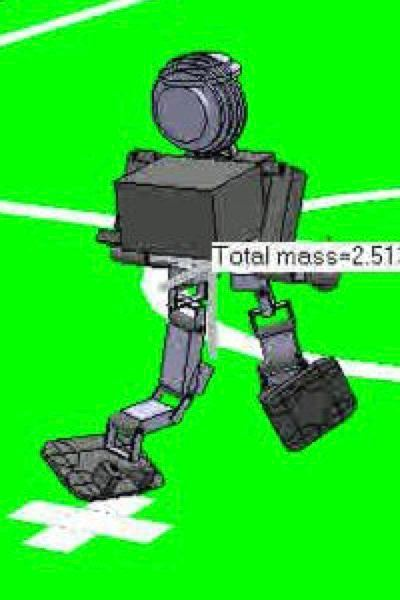
\includegraphics[width=0.3\linewidth]{images/robot_4.5.1.jpg}}
        \hfill
        \subcaptionbox{ \label{fig:robot_4.5.2}}{%
            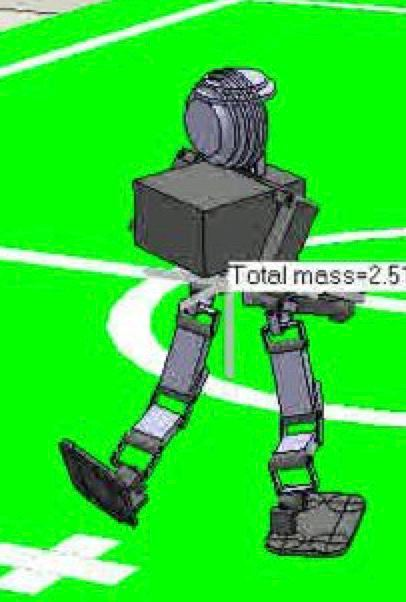
\includegraphics[width=0.3\linewidth]{images/robot_4.5.2.jpg}}
        \hfill
        \subcaptionbox[List-of-Figures entry]{\label{fig:robot_4.5.3}}{%
            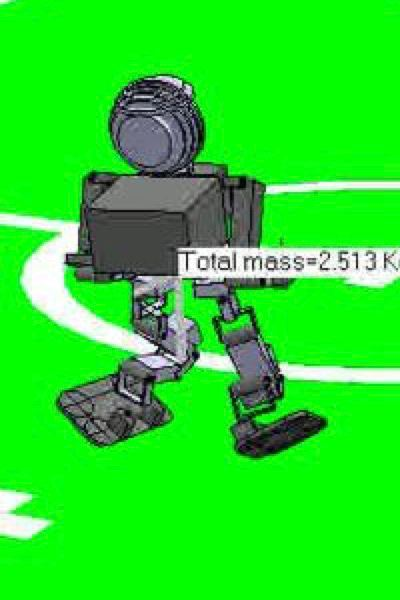
\includegraphics[width=0.31\linewidth]{images/robot_4.5.3.jpg}}
        \hfill
    }
    \caption[Пример ходьбы с ограниченной нагрузкой на сервомоторы]{Пример ходьбы с ограниченной нагрузкой на сервомоторы}\label{fig:robot_4.5}
\end{figure}